
Nesse capítulo, serão apresentados a construção do operador grosso Multiescala e suas aplicaçõesno contexto das equações apresentadas no Capítulo \ref{ch:modelagem}. Daqui para frente, o grid original do problema será denominado grid fino e o operador associado a esse grid $\rigidmatrix$ será chamado de operador fino. A partir do grid fino será construído um grid grosso onde cada elemento é uma aglomeração de elementos do grid fino, o operador associado a esse grid será chamado de operador grosso $\rigidmatrixcoarse$.


O método \textit{Multiscale Finite Element Method} (MSFEM) foi introduzido por \citet{thomashou} e inicialmente foi aplicado para obter soluções aproximadas do grid fino através do grid grosso para casos de transferência de calor de materiais e meios porosos com propriedades aleatórias. A principal conclusão desse trabalho foi que o método MSFEM é capaz de reproduzir a heterogeneidade da solução através da construção das funções de base com solução de problemas locais baseados no operador original. Mais tarde, o método MSFEM se mostrou problemático para conservação de massa em problemas de transporte e, por isso, foram criado os métodos \textit{Mixed Multiscale Finite Element} (MMSFEM) em \citet{mixedmsfem} e  \textit{Multiscale Finite Volume Method} (MSFVM) em \citet{msfv} que garantem a conservação.


Apesar do método MSFVM garantir a conservação da massa, as soluções do grid grosso prolongadas para o grid fino não se mostravam adequadas para todas as situações, assim, foi apresentado o método multiescala iterativo em \citet{iterativems} que ao invés de realizar uma aproximação para a solução fina, utiliza a solução do sistema grosso juntamente com uma relaxação do operador fino para resolver o sistema na malha fina através de iterações de Richardson. A convergência da solução depende da quantidade de vezes que uma relaxação do grid fino é aplicada e varia de problema para problema.

A despeito de todos esses estudos,  o método multiescala continuava sendo aplicado em problemas nos quais informações do grid eram conhecidas para a construção do operador grosso, o que era uma desvantagem em relação ao multigrid algébrico. Essa desvantagem é parcialmente resolvida através do Multiescala algébrico (apresentado em \citet{msalgebrico}) que, de certa forma semelhante aos métodos multigrid algébricos, montam o operador grosso através das entradas da matriz do grid fino utilizando uma ordenação de Wire-Basket que guarda a topologia da malha em questão. Métodos com vários níveis também já foram desenvolvidos como os \citet{multilevel}. \suge{problema nesta citação}


Os trabalhos citados nos parágrafos anteriores são de aplicações do método multiescala para  problemas de fluxo que, historicamente, na indústria do petróleo têm maior apelo por conta da previsão de produção dos campos. Porém, estudos relacionados ao método multiescala para geomecânica também podem ser encontrados em \citet{casteletto}, \citet{irina} e \citet{castelettoacoplado}. É importante salientar que \cite{casteletto} e \cite{irina} apresentam acoplamento entre a simulação de fluxo com a geomecânica. Além disso, visto que \eqref{eq:edp_geomec} é similar ao problema de elasticidade linear para sólidos, podemos encontrar trabalhos utéis com aplicações do método de multiescala neste domínio, por exemplo \citet{mbuck}. 

Implementações em paralelo do método multiescala também podem ser encontradas, por exemplo em \citet{msparalelo} que faz comparação com o método multigrid mostrando que o multiescala é uma opção competitiva e tem escalabilidade similar ao multigrid.

\section{Construção de Operador Grosso Multiescala}

A ideia do método consiste na construção de um operador grosso semelhante ao realizado no multigrid de forma que a solução desse operador pode ser utilizada para ajudar na solução da escala original do problema ou ainda ser utilizada como uma aproximação para a mesma. Para isso, é necessário construir o próprio operador grosso e também operadores que fazem a transferência de escala do grid fino para o grosso (restrição) e do grid grosso para o grid fino (prolongamento).


O primeiro passo para a construção do operador multiescala é gerar um novo grid com menos elementos que o grid original do problema (grid fino), mas que ainda represente o mesmo domínio $\Omega$. Esse novo grid será chamado de grid grosso e as variáveis relacionadas com ele serão assinadas com o sobrescrito $H$.
Dessa forma, o grid grosso possui um conjunto $\coarseelementset$ de elementos onde cada elemento será uma aglomeração de elementos do grid fino. Por exemplo, a Figura \ref{fig:gridgrosso} apresenta um grid grosso $3\times 3$ construído a partir de um grid fino $7\times 7$.  As linhas finas representam as divisões do grid fino e as grossas as divisões do grid grosso, já os  quadrados azuis destacam os nós que pertencem ao grid grosso e ao grid fino simultaneamente. Apesar de serem apresentadas diferentes quantidade de elementos sendo aglomerados para formar o grid grosso, as implementações deste trabalho consideram uma quantidade fixa de elementos em cada direção. Define-se o fator de engrossamento de acordo com \eqref{eq:fatordeengrossamento}. Analogamente podem ser definidos os fatores $\coarsefactorx$ e $\coarsefactory$ que representam os engrossamento em cada direção, onde, $\coarsefactor = \coarsefactorx \times \coarsefactory$.

\begin{figure}[!htbp]
\centering
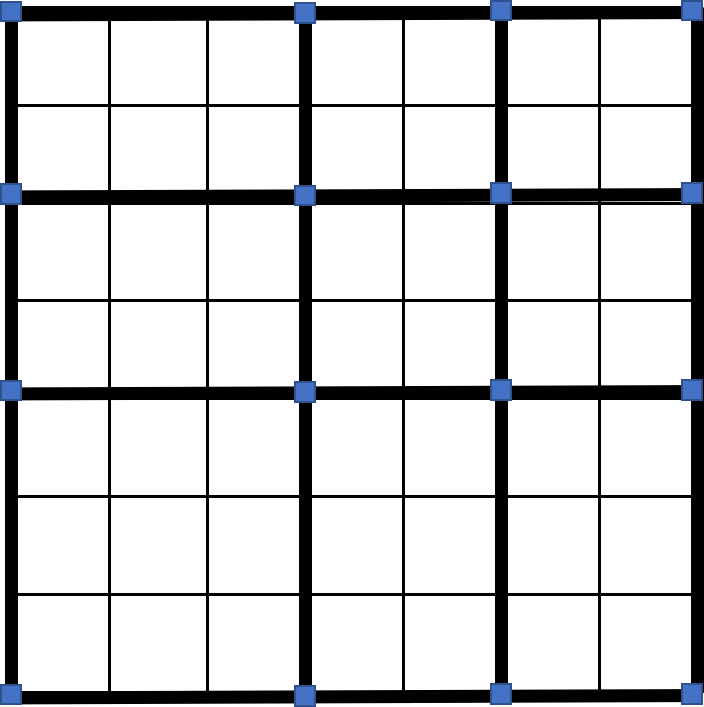
\includegraphics[width=6cm]{chap06/figs/grosso.png}
\caption{Exemplo de grid fino $7\times 7$ e um grid grosso $3\times 3$. O elemento inferior esquerdo é composto por 9 elementos do grid fino enquanto o elemento superior direito é composto com 4 elementos do grid fino.}
\label{fig:gridgrosso}
\end{figure}


\begin{equation} \label{eq:fatordeengrossamento}
    \coarsefactor = \frac{\numelementsfine}{\numelementscoarse}
\end{equation}




Do mesmo modo que apresentado para o grid fino no Capítulo \ref{ch:discretizacao}, cada grau de liberdade grosso $\freedomcoarse$, para $i=1, 2,..., \qtdfreedomcoarse$, será associada a uma função de base $\basefunctioncoarse$ e cada nó associado a uma condição de contorno de Dirichlet $\essentialcoarse$, para i $i=1, 2,..., \qtdessentialcoarse$,  uma função de base $\basefunctioncoarseessential$. E então, é possível encontrar uma solução aproximada no grid fino $\finesolution \approx \msfinesolution$ através de \eqref{eq:aproximacaogrossa}.

\begin{equation} \label{eq:aproximacaogrossa}
    \msfinesolution = \coarsesolution = \sum_{i=1}^{\qtdfreedomcoarse} \basefunctioncoarse \freedomcoarse + {\sum_{i=1}^ {\qtdfreedomcoarse}}  \basefunctioncoarseessential \essentialcoarse
\end{equation}


Diferentemente do caso fino, as funções $\basefunctioncoarse$ serão uma combinação linear das funções $\basefunctionfine$ calculadas a partir de problemas homogêneos locais  para cada elemento $\coarseelement \in \coarseelementset$  apresentados em \eqref{eq:problemaslocais}, conforme proposto em \cite{casteletto}.


\begin{subequations} \label{eq:problemaslocais}
\begin{align}
\sopnabla ^T (D \sopnabla \basefunctioncoarse)  = \mathbf{0} \text{,   em   } \coarseelement \label{eq:operadorlocal}\\
\sopnablafront ^ T ( D  \sopnablafront \basefunctioncoarse) = \mathbf{0}  \text{,   em   } \partial \coarseelement  \label{eq:operadoraresta}\\
\basefunctioncoarse(\mathbf{x}_j) = \delta_{ij} \mathbf{e}
\label{eq:valorvertice}
\end{align}
\end{subequations}
onde $\sopnablafront$ está definido em \eqref{eq:sopnabladef} para as coordenadas $\hat{x}$ e $\hat{y}$ que representam a direção paralela e perpendicular a $\partial \coarseelement$ como mostrada na Figura \ref{fig:direcoesoperadorfronteira}, $\mathbf{x}_j$ representa as coordenadas do vértice relacionado ao grau de liberdade $\freedomcoarse[j]$ e  $\mathbf{e} = [1\quad0]^T $ se $\basefunctioncoarse$ é relacionada a um grau de liberdade x caso contrário,  $\mathbf{e}=[0\quad1]^T$.

\begin{equation}\label{eq:sopnabladef}
\sopnablafront = \begin{bmatrix}
\dxhat  & 0 \\ 
0 & 0 \\ 
0 & \dxhat 
\end{bmatrix}
\end{equation}


%TODO fazer a minha própria figura. Por enquanto está a mesma do casteletto.
\begin{figure}[!htbp]
\centering
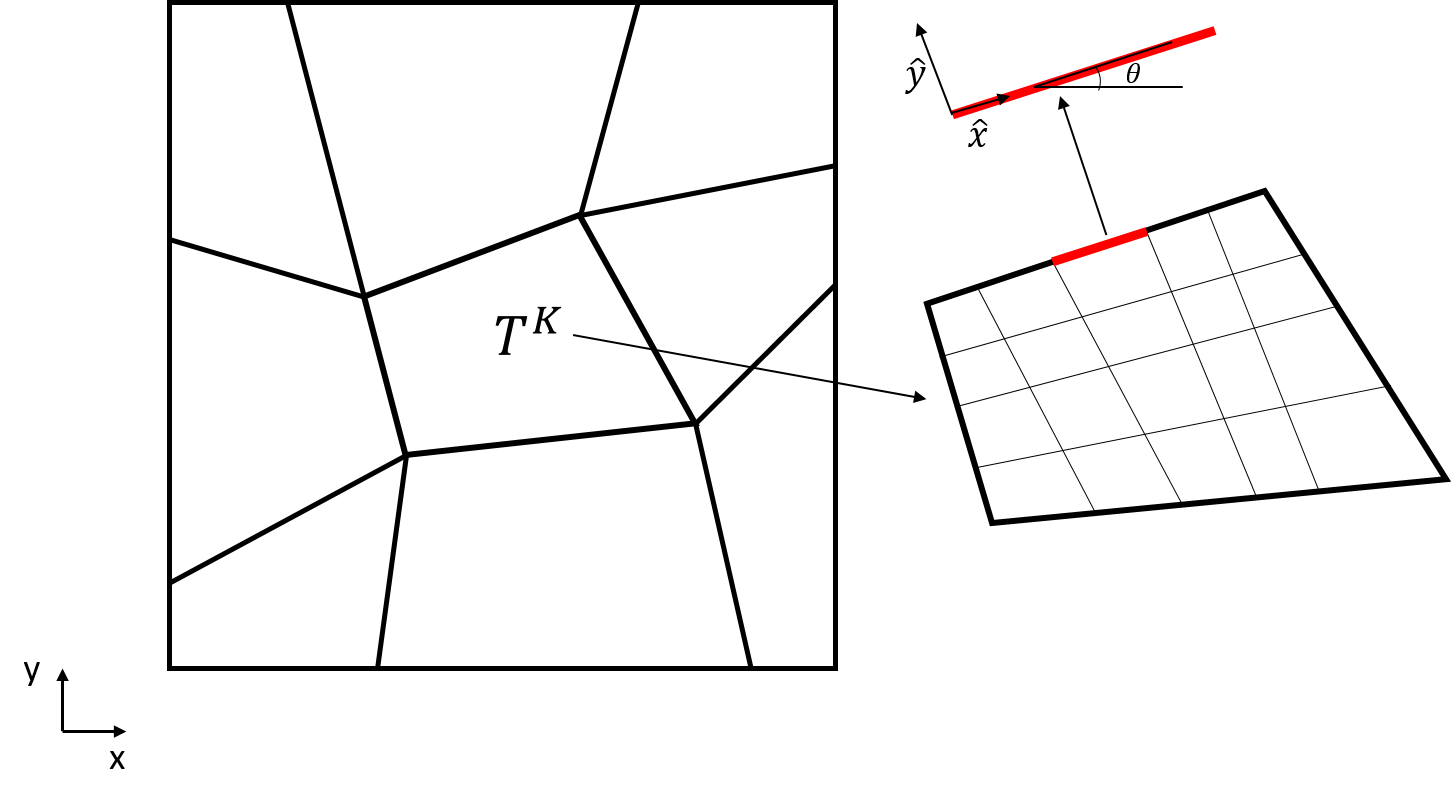
\includegraphics[width=11cm]{chap06/figs/direcoesoperadorfronteira.png}
\caption{Direções para definir operador dos problemas locais na fronteira. Adaptado de \cite{casteletto}.}
\label{fig:direcoesoperadorfronteira}
\end{figure}


Um fato importante é que \eqref{eq:operadorlocal} mostra que a função de base $\basefunctioncoarse$ satisfaz ao mesmo operador que o problema fino, de acordo com \citet{thomashou} essa é uma das vantagens do método multiescala, pois as funções de base tentam reproduzir o operador localmente. Essa vantagem vem com o custo da solução dos problemas locais que também de acordo com \citet{thomashou} são caros. Estimativas do custo desse cálculos são encontradas em \citet{msparalelo} e \citet{mbuck}.

Dessa forma, dado um elemento quadrilátero $\coarseelement$, este possui oito funções $\basefunctioncoarse$ que são não nulas nesse domínio (duas para cada um dos vértices). Considerando uma numeração local do elemento e representando as funções como $\basefunctionelemcoarse$ para $i=1,2,\dots, 8$. A Figura \ref{fig:coarsefunctionslocalnum} apresenta as funções associadas a cada um dos nós na numeração local.


\begin{figure}[!htbp]
\centering
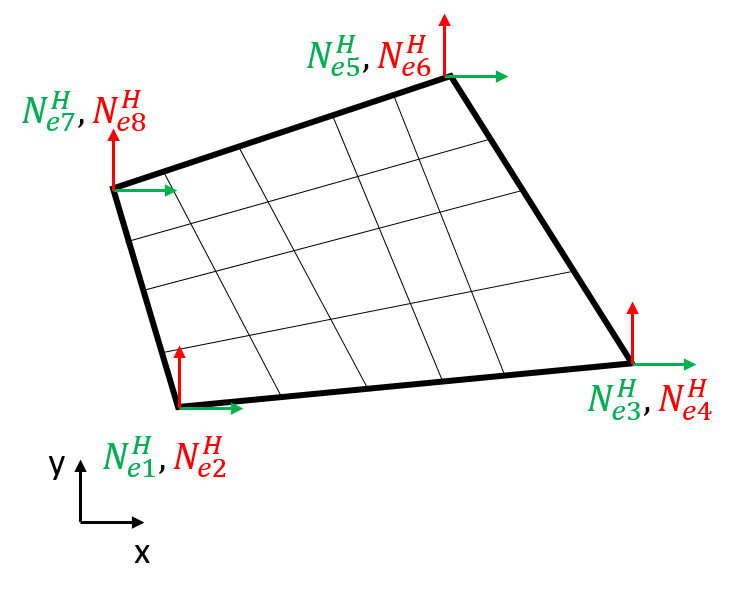
\includegraphics[width=8cm]{chap06/figs/funcoesDeBaseGrossasColorido.png}
\caption{Funções de base associadas a cada um dos nós de um elementos quadrilátero. As cores verdes se referem as funções associadas a x e vermelho a y. As setas representam o valor da função no seu vértice correspondente \eqref{eq:valorvertice}.}
\label{fig:coarsefunctionslocalnum}
\end{figure}

Para cada uma das funções é necessário resolver \eqref{eq:problemaslocais}, a solução é dividida em duas etapas, primeiro é resolvido \eqref{eq:operadoraresta} utilizando como condição de contorno \eqref{eq:valorvertice}, a resposta representa os valores de $\basefunctionelemcoarse$ na fronteira do elemento $\coarseelement$. Essa etapa pode ser realizada utilizando o  método dos elementos finitos onde a matriz relativa a cada elemento, que nesse caso são segmentos de reta, pode ser encontrada no apêndice de \cite{casteletto}. 


Com os valores para  fronteira $\coarseelement$  definidos, eles são utilizados como condição de contorno de Dirichlet para \eqref{eq:operadorlocal}. Esse problema também é resolvido com elementos finitos onde os resultados encontrados serão chamados de coeficientes $p_{ij}$ que descrevem $\basefunctioncoarse$ como combinação linear de $\basefunctionfine$ conforme mostrado em \eqref{eq:linearbasecoarse}. 


\begin{equation} \label{eq:linearbasecoarse}
    \basefunctioncoarse = \sum_{j=1}^{\qtdfreedomfine} p_{ji} \basefunctionfine[j]
\end{equation}


É importante perceber que os coeficientes $p_{ji}$ fazem uma associação entre o espaço grosso e fino. A matriz $\mathbf{P}$ que será o operador de prolongamento terá justamente esses coeficientes como entradas. De forma que, $[\mathbf{P}]_{i,j} = p_{ij}$ e $\mathbf{P}$ tem dimensão $\qtdfreedomfine \times \qtdfreedomcoarse$. A Figura \ref{fig:funcaodebasegrossa} mostra um exemplo de função de base relativa a um grau de liberdade x de um grid grosso construído a partir de um grid $16\times16$ transformado em  $2\times2$. Dois casos são mostrados, um em que as propriedades são constantes e outro em que existe variação no módulo de Young. No caso homogêneo a função tem forma parecida com uma função bilinear padrão de elementos finitos, já no outro caso pode-se perceber alteração na função de base afim de tentar representar as heterogeneidades das propriedades. Além disso, as Figuras \ref{fig:funcaodebasegrossahomy} \ref{fig:funcaodebasegrossahety} mostram a influência dos graus de liberdade x na interpolação do deslocamento em y.



\begin{figure}[]
\center
\subfigure[Logaritmo do Módulo de Young ]{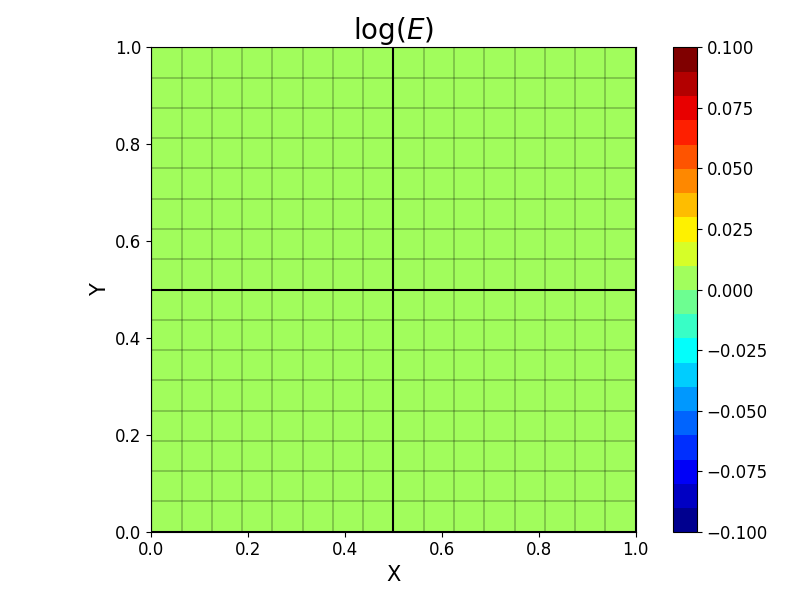
\includegraphics[width=0.45\textwidth]{chap06/figs/CastelettoBases_homogeneo_young.png}}
\qquad
\subfigure[ Logaritmo do Módulo de Young ]{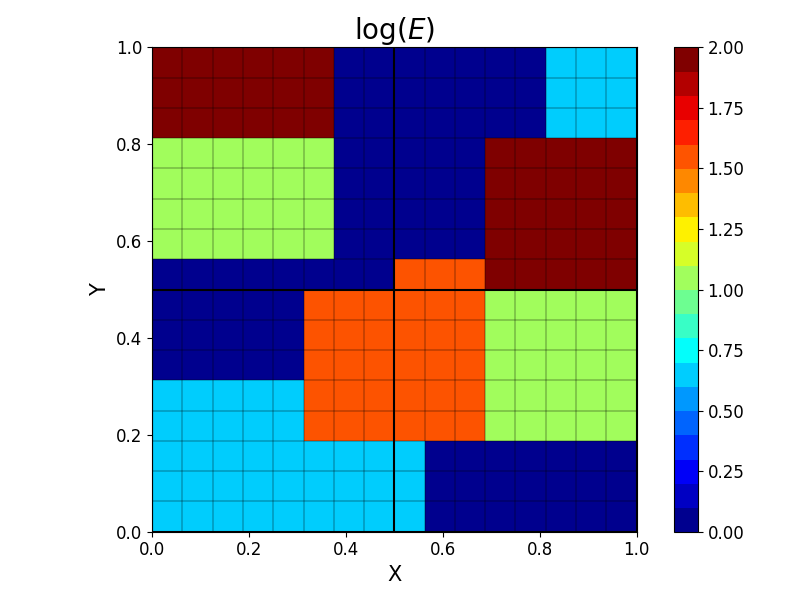
\includegraphics[width=0.45\textwidth]{chap06/figs/CastelettoBases_heterogeneo_young.png}}

\subfigure[ $\mathbf{N}_{i_x}^H$ ]{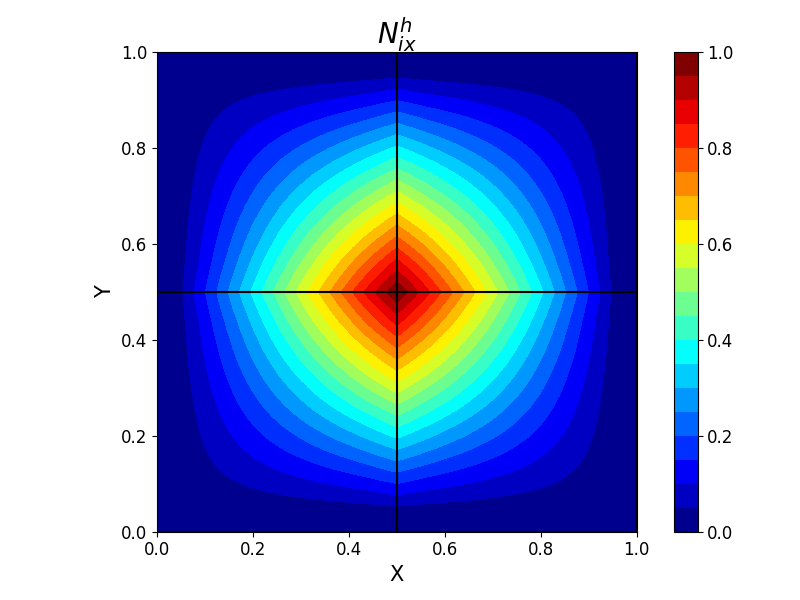
\includegraphics[width=0.45\textwidth]{chap06/figs/CastelettoBases_homogeneo_base_x.png}}
\qquad
\subfigure[ $ \mathbf{N}_{i_x}^H  $ ]{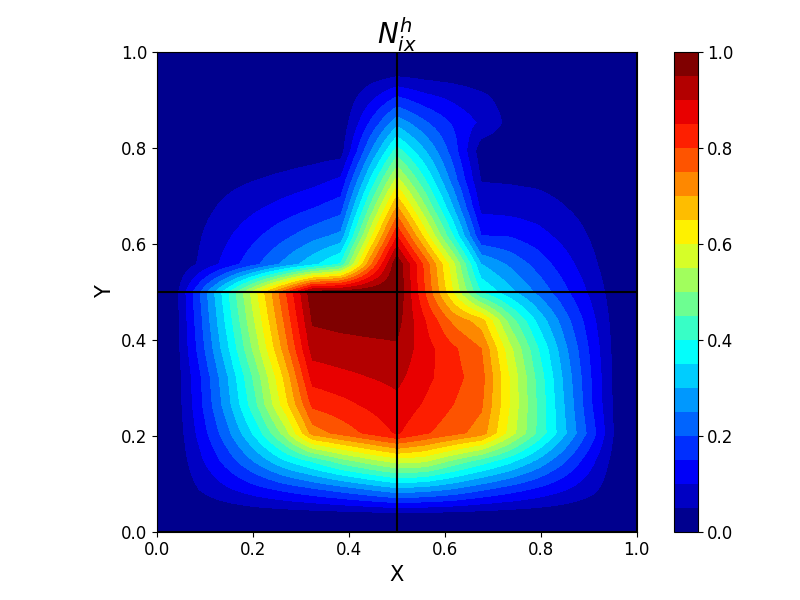
\includegraphics[width=0.45\textwidth]{chap06/figs/CastelettoBases_heterogeneo_base_x.png}}

\subfigure[ $\mathbf{N}_{i_y}^H$ ]{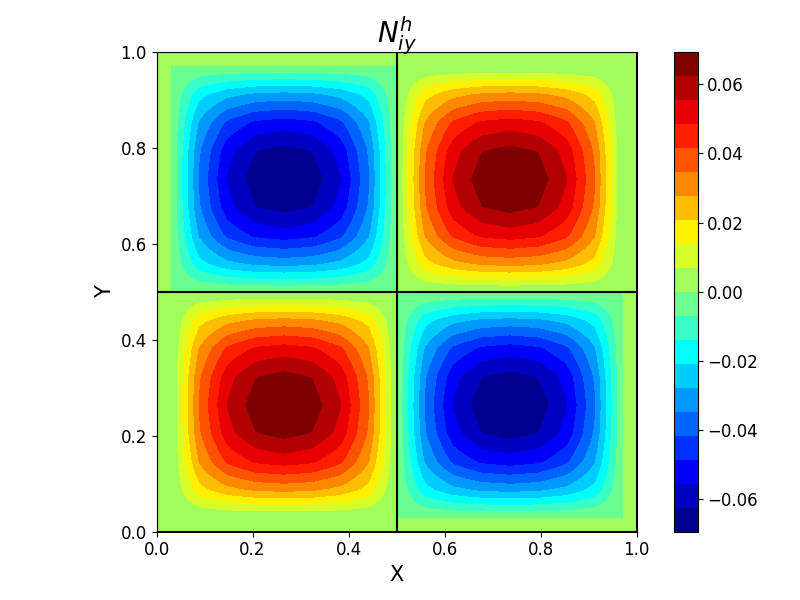
\includegraphics[width=0.45\textwidth]{chap06/figs/CastelettoBases_homogeneo_base_y.png}\label{fig:funcaodebasegrossahety}}
\qquad
\subfigure[ $\mathbf{N}_{i_y}^H$ ]{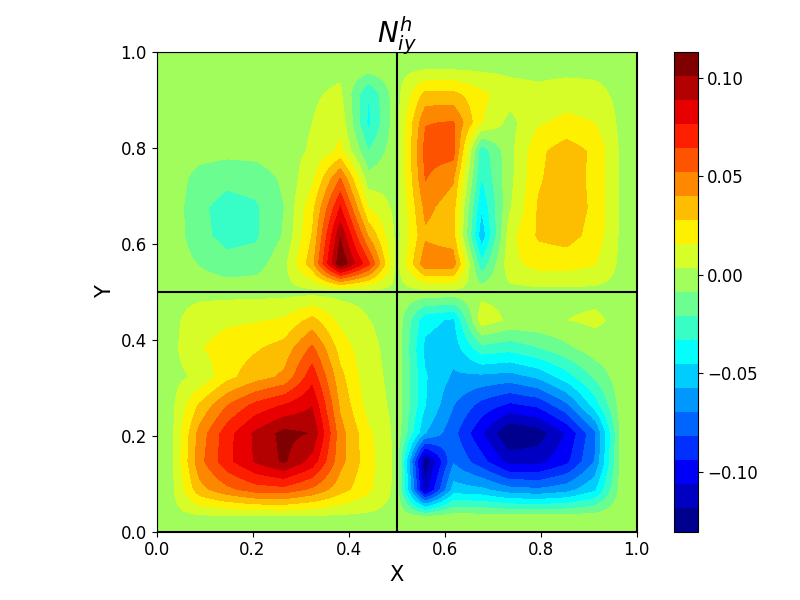
\includegraphics[width=0.45\textwidth]{chap06/figs/CastelettoBases_heterogeneo_base_y.png} \label{fig:funcaodebasegrossahomy}} 

\caption{Exemplo de função de base gerada para módulo de Young homogêneo (lado esquerdo) e para módulo de Young heterogêneo (lado direito). Coeficiente de Poisson considerado constante e igual a 0.2. }\label{fig:funcaodebasegrossa}
\end{figure}


Com \eqref{eq:linearbasecoarse} as funções de base do grid grosso estão determinadas e então é possível formular um novo problema \eqref{eq:weakcoarseformaprox} com espaços $\trialcoarseaprox$ e $\testcoarseaprox$  do grid grosseiro de maneira análoga a realizada em \eqref{eq:weakformaprox}.



\begin{empheq}[box=\mymath]{equation}\label{eq:weakcoarseformaprox}
\begin{split}
\text{Encontrar  }  \mathbf{u} \in \testcoarseaprox \text{ tal que} \qquad \qquad \qquad \qquad \qquad \qquad \qquad \qquad \\
\omeint{ (\sopnabla \mathbf{w})^T D \sopnabla  \mathbf{u}} - \int_{\Gamma_\sigma} \mathbf{w}^T \bar{\mathbf{t}} d\Gamma = (\sopnabla\mathbf{w})^T m P_p \quad \forall \mathbf{w} \in \trialcoarseaprox
\end{split}
\end{empheq}

onde $\trialcoarseaprox =  \text{span}\{ \basefunctioncoarse[1], \basefunctioncoarse[2], \hdots, \basefunctioncoarse[\qtdfreedomcoarse] \}$ e $\testcoarseaprox =  \text{span}\{ \basefunctioncoarse[1], \basefunctioncoarse[2], \hdots, \basefunctioncoarse[\qtdfreedomfine + \qtdfreedomcoarse] \}$. Portanto, analogamente ao grid fino,  a matriz de rigidez relativa ao grid grosso tem entradas dadas por \eqref{eq:entradamatrizgrossa}.

\begin{equation} \label{eq:entradamatrizgrossa}
    \rigidmatrixcoarse_{i,j} =\omeint{(\sopnabla \basefunctioncoarse[i])^T \mathbf{D} \sopnabla \basefunctioncoarse[j]}
\end{equation}

Substituindo \eqref{eq:linearbasecoarse} em \eqref{eq:entradamatrizgrossa}.


\begin{align}
     K^H_{i,j}  & =   \omeint{(\sopnabla \basefunctioncoarse[i])^T \mathbf{D} \sopnabla \basefunctioncoarse[j]} \nonumber \\
                & =   \omeint{(\sopnabla  \sum_{k=1}^{\qtdfreedomfine} p_{ki} \basefunctionfine[k])^T \mathbf{D} \sopnabla( \sum_{l=1}^{\qtdfreedomfine} p_{lj} \basefunctionfine[l] )}  \nonumber \\
                & =    \sum_{k=1}^{\qtdfreedomfine}  \sum_{l=1}^{\qtdfreedomfine} \omeint{p_{ki} ( \sopnabla \basefunctionfine[k])^T \mathbf{D} \sopnabla \basefunctionfine[l] p_{lj}  }                  \nonumber \\
                & =    \sum_{k=1}^{\qtdfreedomfine}  \sum_{l=1}^{\qtdfreedomfine} p_{ki} \left( \omeint{ ( \sopnabla \basefunctionfine[k])^T \mathbf{D} \sopnabla \basefunctionfine[l]   } \right)p_{lj}                            \nonumber \\
                & = \sum_{k=1}^{\qtdfreedomfine}  \sum_{l=1}^{\qtdfreedomfine} \omeint{     p_{ki} \rigidmatrix_{kl} p_{lj}}  \nonumber \\
                & = \sum_{k=1}^{\qtdfreedomfine}  \sum_{l=1}^{\qtdfreedomfine} \omeint{   [P]_{ki} \rigidmatrix_{kl} [P]_{lj}}                                         \nonumber \\
                & = \sum_{k=1}^{\qtdfreedomfine}  \sum_{l=1}^{\qtdfreedomfine} \omeint{   [P^T]_{ik} \rigidmatrix_{kl} [P]_{lj}     }   \label{eq:ptapeinstein}  
\end{align}


Portanto, a \eqref{eq:ptapeinstein} mostra que o operador grosseiro pode ser construído utilizando \eqref{eq:ptap} diferentemente de realizar loop nos elementos grossos para como o realizado pelo método de elementos finitos clássico.

\begin{equation} \label{eq:ptap}
    \mathbf{K}^H = \mathbf{P}^T  \mathbf{K}^h \mathbf{P}
\end{equation}

De forma análoga, pode ser encontrar que a relação entre os lados direito dos dois operador é $\mathbf{f}^H = \mathbf{P}^T \mathbf{f}^h$. Com isso, dado um sistema linear da forma apresentada em \eqref{eq:sistemalinear} é possível encontrar \eqref{eq:aproximacaogrossa2} como aproximação para a solução do grid fino.

\begin{equation} \label{eq:aproximacaogrossa2}
    d^h \approx d^h_{ms} = \mathbf{P} (\mathbf{K}^H)^{-1} \mathbf{P}^{T} \mathbf{f}^h
\end{equation}

Essa aproximação consiste de três passos que são descritas abaixo:

\begin{itemize}
    \item A multiplicação por $\mathbf{P}^T$ representa a restrição do lado direito para o espaço grosseiro.
    \item  o termo $(\rigidmatrixcoarse)^{-1}$ representa o cálculo da solução do espaço grosseiro.
    \item a multiplicação por $\mathbf{P}$ é o prolongamento da solução do espaço grosseiro para espaço fino.
\end{itemize}


Inicialmente, a solução aproximada \eqref{eq:aproximacaogrossa} foi utilizada como solução aproximada para o grid fino em \cite{thomashou}. No caso, tomando como base \eqref{eq:aproximacaogrossa2}, pode-se definir $\preconms = \mathbf{P} (\rigidmatrixcoarse)^{-1} \mathbf{P}^{T}$ como um precondicionador multiescala. Em \citet{zhouiterativo}  essa solução foi utilizada como solver através iterações de Richardson junto com um pré-condicionador do espaço fino, pois mostra que esse pré-condicionador não pode ser utilizado sozinho devido a sua convergência não ser garantida visto que a matriz $\rigidmatrixcoarse$ é deficiente de rank e portanto a matriz de  iteração tem autovalores iguais a um.  Visando reproduzir os resultados para os operadores de elasticidade linear, a Figura \ref{fig:autovaloresRichard} apresenta os autovalores relativos a um caso homogêneo de um grid $40\times40$ para uma iteração de Richardson para quatro diferentes pré-condicionadores: multiescala, ILU(0), multiplicativo (multiescala + ILU(0)) e aditivo (multiescala + ILU(0)). Ainda sobre o fato do operador ser utilizado conjuntamente com um pré-condicionador fino, essa é a abordagem típica e também é utilizada em \cite{casteletto} e \cite{msparalelo}.


\begin{figure}[h]
\center
\subfigure[Multiescala $4\times4$ ]{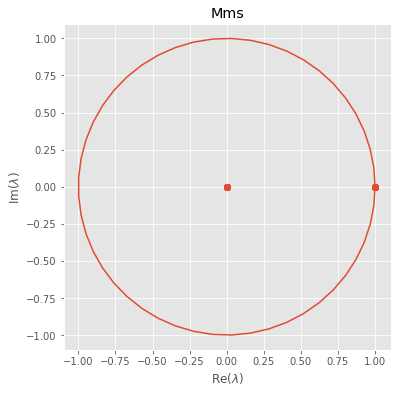
\includegraphics[width=0.45\textwidth]{chap06/figs/autovalores_richardson_mms.png}}
\qquad
\subfigure[ ILU(0) ]{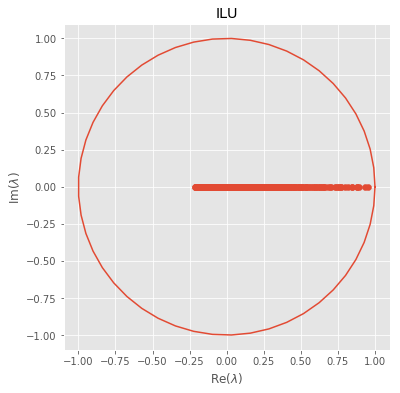
\includegraphics[width=0.45\textwidth]{chap06/figs/autovalores_richardson_ilu.png}}

\subfigure[ Aditivo (Multiescala + ILU(0)) ]{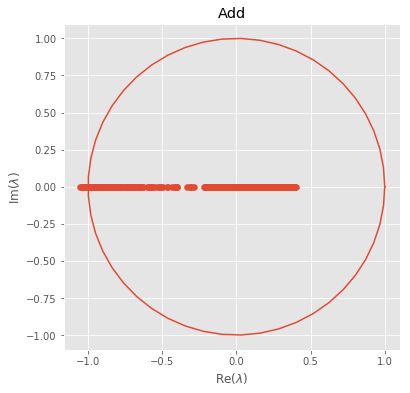
\includegraphics[width=0.45\textwidth]{chap06/figs/autovalores_richardson_aditivo.png}}
\qquad
\subfigure[ Multiplicativo (Multiescala + ILU(0)) ]{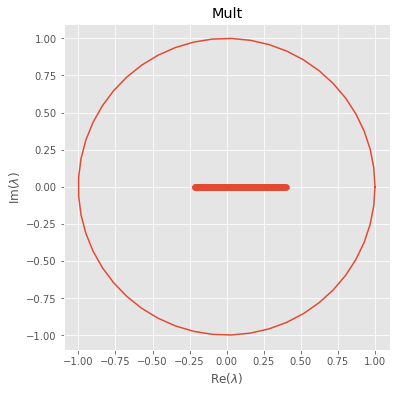
\includegraphics[width=0.45\textwidth]{chap06/figs/autovalores_richardson_multiplicativo.png}}
\caption{Autovalores para matriz de iteração de Richardson para caso homogêneo e isotrópico. Grid de tamanho $40\times40$. }\label{fig:autovaloresRichard}
\end{figure}



Pode-se verificar que o pré-condicionador multiescala não tem convergência garantida, em concordância com a prova mostrada em \cite{zhouiterativo}. O combinativo multiplicativo apresenta bom resultado pois os autovalores aparecem próximos de zero, entretanto, o combinativo aditivo não tem convergência garantida o que mostra que não é interessante utiliza-lo com iterações de Richardson. Ainda sobre isso, \cite{casteletto} mostra que o operador multiplicativo tem melhor desempenho quando utilizado junto com um método de Krylov, naquele contexto utilizando o Bicgstab, do que quando utilizado com o método de Richardson, inclusive, mostra que para várias configurações o solver não consegue convergir. Dado esse resultado, o presente trabalho vai fazer comparações entre os métodos utilizando métodos de Krylov. 

A Figura \ref{fig:autovaloresMatrizPrecon} apresenta os valores da matriz de rigidez pré-condicionada ($\precon \rigidmatrix$) para o mesmo grid de $40 \times 40$, os gráficos apresentam  resultados para engrossamento 2x2, 4x4 e 8x8, todas as figuras são apresentadas com os mesmos eixos para ser possível se observar as espalhamento dos autovalores.

É fato que nos dois casos o aumento do engrossamento causa um maior espalhamento dos autovalores, desse modo é de se esperar que sejam necessárias mais iterações para a convergência do solver. Além disso, o pré-condicionador aditivo possui distribuição pior dos autovalores em relação ao multiplicativo e, portanto, é esperado que utilize mais iterações. Esse aumento tem que ser compensado com uma iteração mais barata por conta da multiplicação matriz vetor.




\begin{figure}[!htbp]
\centering
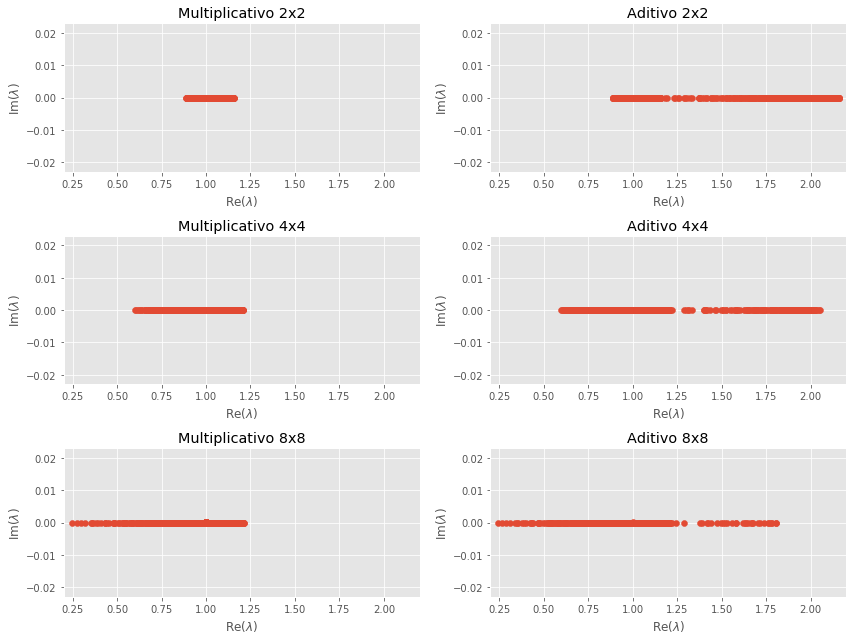
\includegraphics[width=\textwidth]{chap06/figs/AutovaloresMatPrecondicionada.png}
\caption{Autovalores da matriz pré-condicionada para caso homogêneo.}
\label{fig:autovaloresMatrizPrecon}
\end{figure}



\section{Construção do Operador de Prolongamento}

A solução dos problemas locais descritos na seção anterior tem como resultado as entradas $p_{ij}$ do operador em cada um dos elemento de $\coarseelementset$. Para encontrar esses valores é necessário primeiro construir a matriz de rigidez relativa ao elemento em questão que denominaremos de $\rigidmatrixelementms$. Essa matriz será utilizada para a solução de todas as oito funções de base relacionadas com esse elemento, uma maneira de adicionar mais facilmente as condições de contorno nesse caso é utilizar o método de condição de contorno apresentado em \eqref{eq:diagident}, dessa forma, o lado direito do sistema conterá apenas os valores da condição de contorno de Dirichlet que é justamente a solução de \eqref{eq:operadoraresta}.

\vspace{1cm}
\begin{algorithm}[H]
\caption{Cálculo do Prolongamento}
\Inicio{
$\mathbf{P} \leftarrow \mathbf{0}$

\ParaCada{elemento $\coarseelement \in \tau^H$}{
    
    Calcular Matriz de Rigidez $\rigidmatrixelementms$ do Problema Local de $\coarseelement$ 
    
    \Para{$i=1,\hdots,8$}{
    
        Resolver \eqref{eq:operadoraresta} em  $\partial \coarseelement$ com condição de contorno \eqref{eq:valorvertice}
        
        Construa $\mathbf{f}^{\coarseelement}$ com valores da solução do problema de fronteira.
        
        $\mathbf{P_{\text{local}}} \leftarrow  (\rigidmatrixelementms)^{-1} \mathbf{f}^{\coarseelement} $
        
        Atribua em $\mathbf{P}$ o valores $\mathbf{P_{\text{local}}}$ nas posições correspondentes
        
    }
}

}
\end{algorithm}
\vspace{1cm}



Com o algoritmo acima é possível obter $\mathbf{P}$ e, com ele, obter $\rigidmatrixcoarse$ através de \eqref{eq:ptap} e a construção do pré-condicionador $\preconms = \mathbf{P} (\mathbf{K}^H)^{-1} \mathbf{P}^{T}$ fica completa. \eqref{eq:pronlogamento} uma representação do prolongamento onde cada coluna representa uma função de base (essa representação possui um abuso de notação visto que $\basefunctioncoarse$ representa uma função e não entradas da matriz P).



\begin{equation}\label{eq:pronlogamento}
 \mathbf{P} =\begin{bmatrix}
\vdots                    & \vdots                      & \vdots & \vdots   \\ 
 \basefunctioncoarse[1]      & \basefunctioncoarse[2]         & \hdots & \basefunctioncoarse[\qtdfreedomcoarse] \\ 
\vdots                    & \vdots                      & \vdots & \vdots 
\end{bmatrix}
\end{equation}






%O primeiro passo é a construção de um grid grosso a partir do grid fino. A nomenclatura dada para os elementos do grid grosso serão direnciadas da do grid fino pelo sobreescrito H maiúsculo. Isso será feito de forma que cada elemento do grid grosso seja uma aglomeração de elementos do grid fino. Por exemplo, a Figura \ref{fig:gridgrosso} mostra um grid fino 7x7 que foi transformado em um grid grosso 3x3 através da junção de elementos. Nesse caso, o grid grosso é formado por nove elementos e dezesseis nós. Do mesmo que apresentado no Capítulo \ref{ch:discretizacao}, cada grau de liberdade do grid grosso $\freedomcoarse$ terá uma função de base associada  $\basefunctioncoarse$.



%Ele consiste basicamente em construir um operador grosso através do cálculo de funções de base em um grid gerado pelo acoplamento de elementos do grid fino. Pode ser utilizado como pré-condicionador \cite{casteletto}, como solver multinível semelhante aos solver multigrid ou ainda como aproximação para a solução original do problema. Os métodos multiescala tem sido aplicados com sucesso para problemas elípticos que é o caso do problema da elasticidade linear apresentado aqui. As vantagens do método discutido em \cite{thomashou} são que as funções de base multiescala tentam se adaptar às propriedades locais do operador, de forma que o operador grosso as conserve. As funções de base podem ser construídas através da solução de problemas independentes e, portanto, em paralelo.







\section{Cálculo do NNZ do operador de prolongamento}\label{sec:complexProlong}

Em um método multiescala, além da construção de um operador grosso, precisa-se realizar transformações dos vetores entre os espaços fino e grosso  Essas transformações são realizadas através de multiplicação pelos operadores $\mathbf{P}$ e $\mathbf{P}^T$. Essa seção descreve a complexidade destas operações.

As dimensões do operador de prolongamento dependem dos graus de liberdade do operador fino e do  grosso, valendo $\qtdfreedomfine \times \qtdfreedomcoarse$. Conforme visto no Capítulo \ref{ch:sistemas}, a multiplicação de uma matriz esparsa por um vetor é da ordem do número de elementos  não nulos da matriz, assim, apesar de um maior engrossamento do grid reduzir o valor de $n_u^H$,  não necessariamente ocorre  uma redução de elementos não nulos de $P$. Uma motivação para esse fato é que apesar da quantidade de colunas do operador de prolongamento diminuir quando há um engrossamento maior, cada coluna precisa ter uma quantidade maior de não zeros, pois o alcance das funções de base aumenta.

Considerando um grid fino com $\numelementsxfine \times \numelementsyfine$, um grid grosso onde cada elemento tem dimensões $q_x \times q_y$ e, ainda, que mesmo os nós de fronteira com condição de contorno de Dirichlet não são removidos da matriz de rigidez, pode-se encontrar um limite inferior para a não zeros do operador de prolongamento ($\nnzp$) considerando apenas os nós que estão no interior de um elemento grosso. Por exemplo, a Figura \ref{fig:nosinteriores}, mostra os nós interiores das células grossas para um grid $16\times16$ transformado em um grid de $2\times2$. 

\begin{figure}[!htbp]
\centering
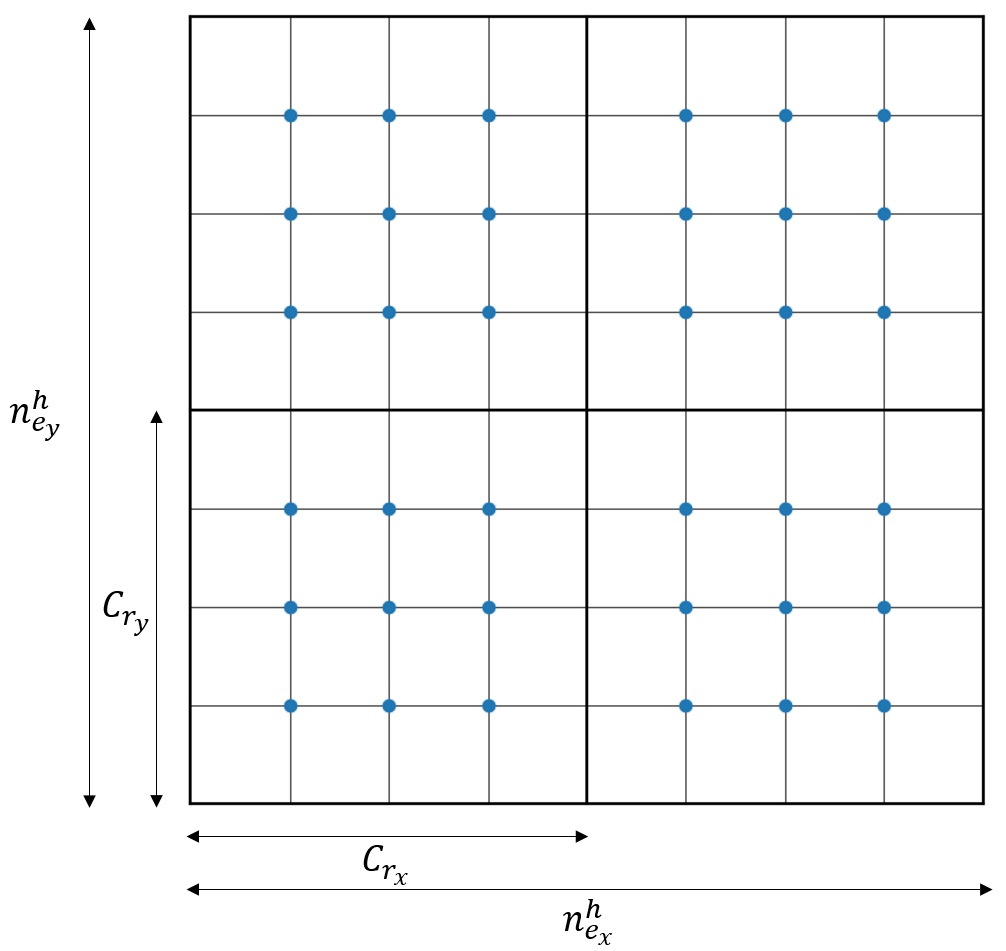
\includegraphics[width=8cm]{chap06/figs/nosinteriores.png}
\caption{Nós interiores dos elementos grossos para um grid fino 8x8 transformado em um grid grosso 2x2.}
\label{fig:nosinteriores}
\end{figure}

No caso, cada célula grossa possui $(q_x-1)(q_y-1)$ nós interiores. Cada um dos dois graus de liberdade de um nó interior recebe influência de cada uma das oito funções de base relacionadas com os vértices do elemento grosso. Dessa forma pode-se escrever \eqref{eq:nnzpraw}.

\begin{equation} \label{eq:nnzpraw}
    \nnzp \ge  \underbrace{(\frac{\numelementsxfine}{q_x} \times \frac{\numelementsyfine}{q_y})}_{\text{qtd. elem. grossos}} \times 8 \times 2 \times (q_x-1)(q_y-1)
\end{equation}

Desenvolvendo,

\begin{align}
     \nnzp   & \ge  16 \times  \frac{\numelementsxfine}{q_x} (q_x-1) \times \frac{\numelementsyfine}{q_y} (q_y-1) \nonumber  \\
                & \ge  16   (\numelementsxfine - \frac{1}{q_x})  (\numelementsyfine - \frac{1}{q_y}) \nonumber   \\
                & \ge  16   (\numelementsxfine - 1)  (\numelementsyfine - 1) \label{eq:nnzp}
\end{align}

Assim, \eqref{eq:nnzp} mostra que $\nnzp$ é no mínimo na ordem do número de elementos do grid fino $\numelementsxfine\times\numelementsyfine$. Um argumento análogo pode ser feito para mostrar que a quantidade de não zeros não é maior que a ordem da quantidade de elementos finos, basta considerar majorar $\nnzp$ considerando que todos os nós são interiores, visto que são eles que tem a maior quantidade de funções de base grossas com valor diferente zero, em comparação com os nós pertencentes as arestas e vértices dos elementos grossos. Dessa forma, pode-se escrever \eqref{eq:nnzprawj}.

\begin{equation}\label{eq:nnzprawj}
    \nnzp \le 8 \times 2 \times \underbrace{(\numelementsxfine + 1)(\numelementsyfine + 1)}_{\text{qtd. nós finos}}
\end{equation}


Portanto, independente do nível engrossamento, a quantidade de não zeros do prolongamento terá não zeros da ordem da dimensão do grid fino. Esse fato é importante, pois, a partir de um certo ponto, não será mais vantajoso engrossar mais o grid por conta do preço dessa multiplicação  que terá sempre que ser pago.